\documentclass[utf8,a4paper,UKenglish,cleveref, autoref, thm-restate]{lipics-v2019}
\usepackage{minted}
\usepackage{stmaryrd}
\usepackage{newunicodechar}
% \usepackage{mathspec} %\usepackage{unicode-math}

\bibliographystyle{plainurl}% the mandatory bibstyle

\newmintinline[icoq]{coq}{}
\newcommand{\mcoq}[1]{\mbox{\icoq{#1}}}

\newcommand\doubleplus{+\kern-1.3ex+\kern0.8ex}
\newcommand\mdoubleplus{\ensuremath{\mathbin{+\mkern-10mu+}}}

\newcommand\bigforall{\mbox{\Large $\mathsurround0pt\forall$}} 

\title{Itauto: an Extensible Intuitionistic SAT Solver} 

%\titlerunning{Dummy short title} %TODO optional, please use if title is longer than one line

\author{Frédéric Besson}{Inria, Univ Rennes, IRISA}{frederic.besson@inria.fr}{}{}
\authorrunning{F. Besson}

\Copyright{Frédéric Besson} %TODO mandatory, please use full first names. LIPIcs license is "CC-BY";  http://creativecommons.org/licenses/by/3.0/


\ccsdesc[500]{Theory of computation~Automated reasoning}
\ccsdesc[500]{Computing methodologies~Theorem proving algorithms}

\keywords{SAT solver, proof by reflection} 

\supplement{\url{https://gitlab.inria.fr/fbesson/itauto}}

\acknowledgements{Thanks are due to Alix Trieu for sharing with us his verified Patricia
  Tree library.  Thanks are also due to Samuel Gruetter for stress testing the
tactic; his feedbacks have been very valuable.}

%\nolinenumbers

%Editor-only macros:: begin (do not touch as author)%%%%%%%%%%%%%%%%%%%%%%%%%%%%%%%%%%
\EventEditors{}
\EventNoEds{0}
\EventLongTitle{}
\EventShortTitle{}
\EventAcronym{}
\EventYear{}
\EventDate{}
\EventLocation{}
\EventLogo{}
\SeriesVolume{}
\ArticleNo{.}
%%%%%%%%%%%%%%%%%%%%%%%%%%%%%%%%%%%%%%%%%%%%%%%%%%%%%%


\begin{document}

\maketitle

\begin{abstract}
  We present the design and implementation of \icoq{itauto}, a Coq
  reflexive tactic for solving intuitionistic propositional logic. The
  tactic inherits features found in modern SAT solvers: definitional
  conjunctive normal form; lazy unit propagation and conflict driven
  backjumping.
  %
  Formulae are hash-consed using native integers thus enabling a
  fast equality test and a pervasive use of Patricia Trees.
  %
  We also propose a hybrid proof by reflection scheme whereby the
  extracted solver calls user-defined tactics on the leaves of the
  propositional proof search thus enabling theory reasoning and the
  generation of conflict clauses.
  %
  The solver has decent efficiency and is more scalable than existing
  tactics on synthetic benchmarks and preliminary experiments are
  encouraging for existing developments.
\end{abstract}


\section{Introduction}
\label{sec:intro}
Using an ideal proof-assistant, proofs would be written at high-level
and mundane proof tasks would be discharged by automated procedures.
%
However, automated reasoning is hard; even more so for
\emph{sceptical}~\cite{HarrisonT98} proof-assistants: generating and
verifying proofs at scale, even for decidable logic fragments, is a
challenge requiring sophisticated implementation strategies.
%
For the Coq proof-assistant, the situation is made slightly worse
because intuitionistic logic is not mainstream for automated provers.
Thus, the Satisfiability Modulo Theory (SMT) approach that is based on a
classical SAT solver needs to be revisited. 

\subsection{Propositional Reasoning and Theory Reasoning in Coq}
\label{sec:prop-in-coq}

There is a variety of Coq tactics which perform intuitionistic
propositional and theory reasoning. We describe here their main
features and explain some limitations, thus motivating the need for a
novel (extensible) solver for intuitionistic propositional logic
(IPL). We defer to Section~\ref{sec:related-work} the discussion of
related approaches rooted in a classical setting and interfacing with
external provers.

\icoq{tauto}~\footnote{\url{https://coq.inria.fr/refman/proof-engine/tactics.html\#coq:tacn.tauto}}
is a complete decision procedure for IPL based on the LJT*
calculus~\cite{Dyckhoff92}.
\icoq{rtauto}~\footnote{\url{https://coq.inria.fr/refman/proof-engine/tactics.html\#coq:tacn.rtauto}}
is another decision procedure for IPL verifying proof certificates
using proof by reflection. %(The manual warns that proof-checking may
%be slower than \icoq{tauto}.)
These decision procedures are usually efficient enough for interactive
use but do not perform theory
reasoning. \icoq{lia}~\footnote{\url{https://coq.inria.fr/refman/addendum/micromega.html\#coq:tacn.lia}}
is a decision procedure for linear arithmetic. It has a classical
understanding of propositional connectives but abstracts away
non-arithmetic
propositions. \icoq{congruence}~\footnote{\url{https://coq.inria.fr/refman/proof-engine/tactics.html\#coq:tacn.congruence}}~\cite{Corbineau06}
does not perform propositional reasoning but decides the theory of
equality with constructors that is useful to reason about inductive
types. Another tactic that is worth mentioning is \icoq{intuition
  tac}~\footnote{\url{https://coq.inria.fr/refman/proof-engine/tactics.html\#coq:tacn.intuition}};
it first performs propositional reasoning and calls the leaf tactic
\icoq{tac} when it gets stuck. (\icoq{tauto} is actually
\icoq{intuition fail}).

In a classical setting, calling a theory solver on the leaves of a
propositional proof search is the basis of the $\mathit{DPLL(T)}$
algorithm~\cite{GanzingerHNOT04}.  Unfortunately, in an intuitionistic
setting, completeness is lost. Example~\ref{exa:incomplete}
illustrates the issue.
\begin{example}[Incomplete Combination]
  \label{exa:incomplete}
  Consider the following goals.
  \begin{minted}{coq}
Lemma Ex1: forall (p:Prop) (x:Z), x = 0 -> (x >= 0 -> p) -> p.
Lemma Ex2: forall (A:Type) (a b c:A), a = b -> b = c -> (a = c -> p) -> p.
\end{minted}
  For \icoq{Ex1} and \icoq{Ex2}, \icoq{intuition lia} (resp. \icoq{intuition congruence}) fail whereas
  the goal can be decided using a combination of
  propositional logic with the theory of linear arithmetic and
  the theory of equality, respectively.
  %
  The reason is that the \icoq{intuition} part does nothing and
  therefore calls the leaf tactic on the unmodified goal.  For
  \icoq{Ex1}, \icoq{lia} abstracts away non-arithmetic
  propositions\footnote{The propositional variable \icoq{p} is replaced by
    \icoq{True} or \icoq{False} depending on its polarity.} and is
  left with the non-theorem
  \begin{minted}{coq}
    x = 0 -> (x >= 0 -> True) ->  False.
  \end{minted}
  For \icoq{Ex2}, \icoq{congruence} abstracts away
  propositions and is also left with a non-theorem:
  \begin{minted}{coq}
    a = b -> b = c -> False.
  \end{minted}
\end{example}
Besides completeness, \icoq{intuition tac} has also an efficiency issue and may call the leaf tactic \icoq{tac}
%In term of efficiency, \icoq{intuition tac} does not \emph{learn}
%conflict clauses and therefore may call the leaf tactic \icoq{tac}
more often than necessary. %If the leaf tactic is costly, this has a negative effect on efficiency.
This is illustrated by Example~\ref{ex:too-many-calls}.
\begin{example}[Spurious Leaf Tactic Call]
  \label{ex:too-many-calls}
  Consider the following goal.
  \begin{minted}{coq}
Lemma Ex3: forall (A:Type) (x y:A) (p q:Prop),
                  x = y -> p \/ q -> (p -> y = t) -> (q -> y = t) -> x = t.
  \end{minted}
  In this case, \icoq{intuition congruence} performs a case-split
  over \icoq{p\/q}, and derives \icoq{y=t} by
  \emph{modus-ponens}. Eventually, it calls the leaf tactic
  \icoq{congruence} twice.  However, in both branches,
  \icoq{congruence} solves the same theory problem \emph{i.e.},
  \icoq{x = y -> y = t -> x = t}.
\end{example}

\subsection{Contribution}

A contribution is the design and implementation of a reflexive
intuitionistic SAT solver in Coq.  The SAT solver obtains decent
performances using features found in state-of-the-art SAT solvers such
as hash-consing, lazy unit propagation, backjumping and theory
learning. It also makes a pervasive use of native integers and
Patricia Trees.


Another contribution is a variation of the proof by reflection
approach where the verified extracted SAT solver is first run inside
the proof engine. This enables to increase the expressiveness by
calling user-defined tactics on the leaves of the propositional proof
search thus allowing theory reasoning.
%
We extract unsat cores by inspecting the proof terms generated by the
user-provided tactic. The unsat core is then injected in the SAT
solver as a novel propositional clause. To our knowledge, this design
combining reflexive code with tactics is original. Besides increased
flexibility, another advantage is to factorise the code and localise the
soundness bugs to its unverified part.

The rest of the paper is organised as follows.
%
In Section~\ref{sec:design}, we present the main features of our SAT
solver and its implementation in Coq.
%
The structure of the soundness proof is detailed in Section~\ref{sec:reflection}.
%
In Section~\ref{sec:reflection}, we explain how to interface the SAT
solver with the proof engine and  user-defined
tactics.
%
We show experimental results in Section~\ref{sec:experiments} where we
compare with the existing Coq tactics.
%
Related work is presented in Section~\ref{sec:related-work} and
Section~\ref{sec:conclusion} concludes.

Note that the code snippets in the paper have been edited and
idealised for clarity. 

\section{Design of an Intuitionistic SAT solver}
\label{sec:design}

Our algorithm is reusing several key components of modern SAT
solvers. Fortunately, they are only slightly adapted to the
intuitionistic setting.

\subsection{Syntax and Semantics of Formulae}
\label{sec:syntax}
Our SAT solver takes as input hash-consed~\cite{Allen-hcons} formulae defined by the inductive type \icoq{LForm}.
\begin{minted}{coq}
Inductive LForm : Type :=
| LFF
| LAT : int -> LForm
| LOP : lop -> list (HCons.t LForm) -> LForm
| LIMPL : list (HCons.t LForm) ->  (HCons.t LForm)  -> LForm.
\end{minted}
The syntax is mostly standard and models n-ary propositional operators.
%
\icoq{LFF} represents the proposition \icoq{False}. 
\icoq{LAT i} represents the propositional variable \icoq{pi}.
%
\icoq{LOP o} $[f_1; \dots; f_n]$ where \icoq{o} $\in$\{\icoq{AND},
\icoq{OR}\} represents a n-ary conjunction or disjunction.
%
\icoq{LIMPL} $[f_1; \dots; f_n]$ $f$ represents a n-ary implication
with $f_1$, \dots, $f_n$ being the premisses and $f$ the conclusion.
%
All sub-formulae are hash-consed \emph{i.e.} \icoq{f:HCons.t LForm}
is a pair made of a formula and a unique index.
%
Because it enables a fast equality test of formulae in $O(1)$, hash-consing is essential for efficiency.
%
N-ary operators allow for a sparser conjunctive normal form (see \emph{e.g.}~\cite{LescuyerC09}).

The interpretation of a formula \icoq{f:LFORM} is given by structural recursion with respect
to an environment \icoq{e:int -> Prop} mapping indexes \emph{i.e.}, propositional variables, to
propositions.
\[
  \begin{array}{lcl}
    \llbracket \mcoq{LFF} \rrbracket_e &=& \mcoq{False} \\
    \llbracket \mcoq{LAT}\ i \rrbracket_e &=& e\ i \\
    \llbracket \mcoq{LOP}\  \mcoq{AND}\ [f_1;\dots;f_n] \rrbracket_e &=& \llbracket f_1 \rrbracket_e \land \dots\land \llbracket f_n \rrbracket_e\\
    % \bigwedge_{i\in [1;n]} \llbracket f_i \rrbracket_e \\
    \llbracket \mcoq{LOP}\  \mcoq{OR}\  [f_1;\dots;f_n] \rrbracket_e &=& %\bigvee_{i\in [1;n]} \llbracket f_i \rrbracket_e \\
    \llbracket f_1 \rrbracket_e \vee \dots\vee \llbracket f_n \rrbracket_e\\
    \llbracket \mcoq{LIMPL}\ [f_1;\dots;f_n]\  f \rrbracket_e &=& \llbracket f_1\rrbracket_e \rightarrow \dots \rightarrow \llbracket f_n \rrbracket_e \to \llbracket f \rrbracket_e \\
  \end{array}
\]
In the following, as the environment $e$ is fixed, we drop the
subscript and write $\llbracket f \rrbracket$ for $\llbracket f \rrbracket_e$.

\subsection{Intuitionistic Clausal Form}


%\subsubsection{Design Principles}
In a classical setting, to prove that a formula $f$ is a tautology, a modern
SAT solver proves that the conjunctive normal form (CNF) of the
negation of $f$ is unsatisfiable. In other words, a SAT solver
exploits the fact that $\neg (\neg f)$ is equivalent to $f$ and that
the CNF conversion preserves provability.
%
In an intuitionistic setting, this approach is not feasible because
\emph{reductio ad adsurdum} is not logically sound and
the usual CNF conversion requires De Morgan laws which do not hold either.
%
Yet, Claessen and Rosén~\cite{ClaessenR15} show that it is possible to
transform an intuitionistic  formula $f$ into an equi-provable formula of the form
\[
  \bigwedge F \land \bigwedge I \to q
\]
where $q$ is a variable ; $f \in F$ is a so-called \emph{flat clause} of the
form $p_1 \to \dots p_n \to q_1 \lor \dots \lor q_m$ where the $p_i$
and $q_i$ are variables and $i\in I$ is a so-called \emph{implication clause}
of the form $(a\to b) \to c $ where $a$, $b$ and $c$ are variables.
%
The transformation is based on Tseitin definitional CNF~\cite{Tseitin1983} with the
modification that a clause is written
$p_1 \to \dots \to p_n \to q_1 \lor \dots \lor q_n$ instead of
$\neg p_1 \lor \dots \neg p_n \lor q_1 \dots q_n$.
%
The \emph{implication clauses} are reminiscent of the fact that double
arrows (\emph{e.g.}, in the LJT proof system) need a
treatment that is specific to intuitionistic logic. %In particular, the set of flat clauses
%$(a\lor c) \land (b \to c)$ is only equivalent in a classic setting.

Our implementation is along these lines but optimises the
transformation in order to reduce both the set of \emph{flat clauses}
and \emph{implication clauses}.  To reduce the set of \emph{flat
  clauses}, our definitional CNF is based on Plaisted and Greenbaum
CNF~\cite{PlaistedG86} which exploits the polarity of formulae and is
tabulated thus avoiding recomputing the CNF of identical sub-formulae.
%
In order to reduce the set of \emph{implication clauses}, we exploit
the fact that, if the conclusion $q$ is decidable, intuitionistic logic reduces to
classical logic. In that case, it is therefore
admissible to replace an \emph{implication clause} $(a \to b) \to c$
by the equivalent \emph{flat clauses} $(a\lor c) \land (b \to c)$.
%
Moreover, before performing CNF conversion, formulae are flattened
using the associativity of $\land$ and $\lor$. This has the advantage
of augmenting the arity of the operators, reducing the depth of the
formulae, and therefore reducing the number of intermediate propositional variables.

\subsubsection{Pre-processing}
The input formula is only using binary operators.  To obtain n-ary
operators, we recursively apply the following equivalences (the
operator $\doubleplus$ is the concatenation of lists):
\[
  \begin{array}{lcl}
    \mcoq{LOP OR}\ (\mcoq{LOP OR}\ l_1):: l_2 &=& \mcoq{LOP OR}\ (l_1 \doubleplus l_2)\\
    \mcoq{LOP AND}\ (\mcoq{LOP AND}\ l_1):: l_2 &=& \mcoq{LOP AND}\ (l_1 \doubleplus l_2)\\
    \mcoq{LIMPL}\ (\mcoq{LOP AND}\ l_1):: l_2\  r  &=& \mcoq{LIMPL}\ (l_1 \doubleplus l_2)\ r\\
    \mcoq{LIMPL}\ l_1 (\mcoq{LIMPL} l_2\ r)  &=& \mcoq{LIMPL}\ (l_1 \doubleplus l_2)\ r\\
  \end{array}
\]

\subsubsection{Literals}
Tseitin style CNF consists in introducing fresh
propositional variables.  In a proof-assistant, modelling freshness
may incur some proof overhead. Fortunately, in our case, the new
propositional variables are not arbitrary but correspond to
sub-formulae. As a result, we represent a propositional variable by a
hash-consed formula (\icoq{HFormula} = \icoq{HCons.t LForm}) and a
literal is a positive or negative hash-consed formula.
\begin{minted}{coq}
Inductive literal : Type := | POS (f: HFormula) | NEG (f: HFormula)
\end{minted}
As usual, a clause is a list of positive and negative literals but with the following interpretation.
\[
  \begin{array}{lcl}
    \llbracket \icoq{NEG} f :: l \rrbracket_e & = & \llbracket f \rrbracket_e \rightarrow \llbracket l \rrbracket_e \\
    \llbracket \icoq{POS} f :: l \rrbracket_e & = & \llbracket f \rrbracket_e \lor \llbracket l \rrbracket_e \\
    \llbracket [] \rrbracket_e &= & \icoq{False} \\
  \end{array}
\]

\subsubsection{Introduction Rule}
Before running the CNF conversion \emph{per se}, we inspect the
formula and perform \emph{reductio ad adsurdum} if possible. The
function \icoq{intro_impl} performs the introduction rule for
implication with the twist that the conclusion is double negated if it
is decidable. Therefore, \icoq{intro_impl: HFormula -> (list literal * HFormula)}
takes as input a hash-consed formula and returns a pair
$(l,c)$ where $l$ are hypotheses and $c$ is the conclusion.
%%where
%%\icoq{None} indicates that the conclusion is \icoq{False} thus
%%enabling classical reasoning.
\begin{minted}{coq}
intro_impl (LIMPL  l r) = if is_dec r
                          then ((NEG r):: map POS l , HLFF)
                          else (map POS l, r)
intro_impl f   = if is_dec f then ([NEG f] , HLFF) else ([], f)
\end{minted}
The constant \icoq{HLFF} is the hash-consed formula \icoq{LFF}
\emph{i.e.}, the syntax for the proposition \icoq{False}.  The
\icoq{is_dec} predicate is implemented by a boolean flag
stored together with the hash-cons of the formula. It is recursively
propagated from atomic propositions that are known to be classical
\emph{i.e.}, we have $r \lor \neg r$.

\subsubsection{Construction of the CNF}
The next step consists in computing the CNF of the literals and of the
formula in the conclusion.  We recursively compute for a positive literal
\icoq{CNF-} \emph{i.e.}, clauses for the elimination rule; and for a
negative literal (or the conclusion) \icoq{CNF+} \emph{i.e.}, clauses
for the introduction rule.
\[
  \begin{array}{cc}
  \icoq{AND-} \dfrac{ f = (f_1 \land \dots f_n) }
  { (f \to f_1) \land \dots \land (f \to f_n) } &
    %
    \icoq{AND+} \dfrac{ f = (f_1 \land \dots f_n) }
    { f_1 \to \dots \to f_n \to f } \\\\
    %
    \icoq{OR-}  \dfrac{ f = (f_1 \lor \dots f_n) }
    { (f \to f_1 \lor \dots f_n) } &
    %
    \icoq{OR+}  \dfrac{ f = (f_1 \lor \dots f_n) }
    { (f_1 \to  f) \land  (f_n \to f) }\\\\
    %
    \icoq{IMPL-}  \dfrac{ f = (f_1 \to \dots \to f_n \to r) }
                   { (f \to f_1 \to \dots \to f_n \to r) } &
    % 
    \icoq{IMPL+}  \dfrac{ f = (f_1 \to \dots \to f_n \to r) }
                   { (r \to f) \land \bigwedge_{(\icoq{is_dec}\ f_i)} (f_i \lor f)   }\\\\
  \end{array}
\]
Except for \icoq{IMPL+}, the CNF is complete and all the formulae are
both classical and intuitionistic tautologies.
%
For \icoq{IMPL+}, if not all the $f_i$ are classical propositions, the
clausal encoding is partial and we also generate the \emph{implication
  clause} $(f_1 \to \dots \to r) \to f$. Note that, if the conclusion
is \icoq{False}, we also generate the full clausal form for 
\[
  I = (r \to f) \land (f_1 \lor f) \land \dots \land (f_i \lor f)
\]
This is sound because $I \to \icoq{False}$ is an intuitionistic tautology.% for ($f = (f_1 \to \dots \to f_n \to r)$).

\subsection{Lazy Unit Propagation}

Once a clause is reduced to a single literal, say $l$, \emph{unit
  propagation} simplifies all the remaining clauses using $l$. There
are three cases to consider.  If a clause $c$, does not mention $l$,
it is left unchanged. If the literal $l$ belongs to the clause $c$,
the clause is redundant and it is removed (see \icoq{R1} and
\icoq{R2}). If the negation of the literal $l$ belongs to the clause,
we deduce the simplified clause $c \setminus \neg l$ (see \icoq{M1} and \icoq{M2}). In logic terms,
we have the following inferences:
\[
  \icoq{R1}\dfrac{ p }{ p \lor r } \qquad
  \icoq{R2}\dfrac {\neg p }{ p \to r } \qquad 
  \icoq{M1}\dfrac{p \quad p \to r}
  { r }  \qquad
  \icoq{M2}\dfrac{\neg p \quad p \lor r}{r} 
  \qquad
\]


A naive algorithm linearly traverses every clause and is therefore inefficient.
%
A key observation is that the purpose of unit propagation is
to produce new unit clauses. Said otherwise, it not necessary to traverse
clauses with at least 2 literals that are not assigned.
%% By indexing
%% clauses on these two literals, unit propagation can be implemented
%% more efficiently.
%
We implement a variant of head-tail
lists~\cite{Zhang96anefficient,ZhangS00} that is simpler than the
2-watched literals optimisation~\cite{MoskewiczMZZM01}.
%
Moreover, as functional lists do not provide a constant-time access to the
tail of a list, instead of head-tail lists, we have 2-heads lists.
%
A clause that is neither the empty clause nor the unit clause is
represented by the type \icoq{watched_clause} given below.
\begin{minted}{coq}
Record watched_clause := {
  watch1 : literal;
  watch2 : literal;
  unwatched: list literal }.
\end{minted}
Watched clauses are indexed on their watched literals but also on whether the leading literals are positive or negative.
%
To get an efficient representation of sets of clauses, they are indexed and stored in Patricia Trees~\cite{Okasaki98fastmergeable}. 
%
In order to implement so-called \emph{non-chronological backtracking} (see Section~\ref{sec:case-split}),
we also track the set of literals that are needed to deduce a clause. As a
result, each clause is annotated  with a set of literals \icoq{LitSet.t} that is also
represented using Patricia Trees.
\begin{minted}{coq}
  Record Annot (A: Type) := { elt := A ; deps := LitSet.t }
\end{minted}
Therefore, unit propagation
operates on the following \icoq{watch_map} data-structure.
\begin{minted}{coq}
Definition clause_set := ptrie (Annot watched_clause).
Definition watch_map  := ptrie (clause_set * clause_set).
\end{minted}
A \icoq{watch_map} $m$ maps a propositional variable $f$ \emph{i.e.},
a hash-consed formula, to two sets $(n,s)$ of clauses where clauses in $n$ are watched by $\icoq{NEG}\ f$ and clauses in $p$ 
are watched  by $\icoq{POS}\ f$. More precisely, we have
\[
  \begin{array}{lcl}
    c \in n &\mathit{ iff }& c.watch1=\icoq{NEG}\ f \lor c.watch2=\icoq{NEG}\ f \\
    c \in p &\mathit{ iff }& c.watch1=\icoq{POS}\ f \lor c.watch2=\icoq{POS}\ f \\
  \end{array}
\]
Suppose that we perform unit propagation for the literal
$\icoq{POS}\ f$ for a \icoq{watched_map} $m$ such that $m[f] = (n,p)$.
The clauses in $p$ are redundant and can be dropped; the clauses in $n$
need to be processed and reduced. The reduction takes as argument the
set of literals that are already assigned, a watched clause $c$ and
returns an annotated clause \icoq{Annot clause} where the type
\icoq{clause} is given below
\begin{minted}{coq}
Inductive clause:=
 | EMPTY  
 | TRUE
 | UNIT (l:literal)
 | CLAUSE (wc:watched_clause)
\end{minted}
\icoq{EMPTY} represents the \emph{empty} clause, \emph{i.e.} a
contradiction. In that case, unit propagation concludes the proof.
%
\icoq{TRUE} represents a redundant clause that will be dropped.
%
\icoq{UNIT l} is a unit clause to be propagated and \icoq{CLAUSE wc} is a watched clause.

Without loss of generality, suppose that $f$ belongs to the set of assigned
literals \icoq{s} and that we have a clause $c$ has the form:
\[
  c = \{| \icoq{watch1} := \neg f ; \icoq{watch2} := x ; \icoq{unwatched} := [\neg y_1;\neg y_2;\dots;\neg y_n]|\}
\]
The \icoq{reduce} function takes as input the watched literal $x$ and aims at finding in the list
$[\neg y_1;\neg y_n;\dots;\neg y_n]$ a watched literal $y_i$ (\emph{i.e.}, $y_i$ is not assigned in \icoq{s})
and return as clause the rest of the
list. %The argument \icoq{d} is used to record the literals in the
%clause that are known to be assigned.
\begin{minted}[escapeinside=\#\#,mathescape=true]{coq}
  reduce s d x [] = {| elt := UNIT x ; deps := d |}
  reduce s d x (y::l) = {| elt := TRUE ; deps := d |} when y #$\in$# s
  reduce s d x (y::l) = reduce s ((deps (s y)) #$\cup$# d) l when #$\neg$# y #$\in$# s
  reduce s d x (y::l) =
    let wc := {| watch1 := x ; watch2 := y ; unwatched := l |} in
    {| elt := CLAUSE wc ; deps := d |} when y #$\notin$# s
\end{minted}
If the list is empty, we have produced the unit clause $x$ and unit
propagation will be recursively called.  Let $y$ be the head of the list
$l$.  If $y$ is not assigned in the environment $s$, we return a
novel clause where the watched literals are $x$ and $y$.
%
If $y$ is already assigned with the same polarity in $s$, the clause
is redundant and can be dropped.  If $y$ is already assigned but with
opposite polarity ($\neg y \in \icoq{s}$), the reduction is recursively called threading along
the dependencies of the literal $y$.
%
\begin{example}
  Suppose that the set of assigned literals is given by
  $\icoq{s} = \{ f; y_1; y_n \}$ and we perform unit
  propagation over the clause $c$.  By construction, we know that
  neither $x$ nor $\neg x$ are assigned in $\icoq{s}$. To get a
  well-defined watched clause with 2 watched literals, we need to find
  a replacement for the literal $\neg f$ in the list
  $[\neg y_1;\neg y_2;\ldots;\neg y_n]$.
  %
  As $\{y_1, y_n\} \subseteq  \icoq{s}$, a greedy unit propagation would deduce that
  $\neg y_1$ and $\neg y_n$ can be removed but as the prohibitive cost of a linear scan of the whole clause.
  The idea of lazy unit propagation is to stop at the first unassigned literal \emph{i.e.} $y_2$.
  Therefore, we generate the watched clause
  \[
    \{ \icoq{watche1} := x ; \icoq{watche2} := \neg y_2 ; \icoq{unwatched} := [\neg y_3;\dots;\neg y_n] \}
    \]
    In logic terms, we have performed the following \emph{modus ponens} ignoring $y_n$
    \[
      \dfrac{
        f \quad y_1 \quad f \to x \to y_1 \to y_2 \to \dots  \to y_n \to \icoq{False}
      }
      {  x \to y_2 \to \dots \to y_n \to \icoq{False} }
    \]
\end{example}


\subsection{Case Splitting and Backjumping}
\label{sec:case-split}

When all the unit clauses are propagated, the solver performs a
case-split over a clause. The clause needs to represent a
disjunction. If the conclusion is \icoq{False}, any clause may be
selected. Otherwise, the clause may only contain  either positive literals or  negative
\emph{classical} literals. The soundness of this argument is expressed by
the following propositional equivalences.
\[
  \begin{array}{l}
  (\bigwedge_i p_i \to \bigvee_j q_j) \to \bot \equiv (\bigvee_i \neg p_i \lor \bigvee_j q_j) \to \bot\\
    \bigwedge_i (p_1 \lor \neg p_i) \to ((\bigwedge_i p_i \to \bigvee_j q_j) \to g) \equiv (\bigvee_i p_i \lor \bigvee_j q_j) \to g
  \end{array}
\]
A naive algorithm consists in doing a recursive call for each literal,
say $l_i$, of the clause.  However, if for one of the cases, the proof
does not depend on the literal $l_i$, it is sound to ignore the other
cases and immediately return (\emph{backjump}) to a previous
case-split. This is illustrated by Example~\ref{exa:backjump}.
\begin{example}[Backjumping]
  \label{exa:backjump}
  Consider the following goal where each clause $H_i$ is tagged with a
  set of dependencies $d_i$ where the $d_i$ are disjoint and do not
  contain the literals $\{l,m,n,o\}$.
  \[
    H_1 : (l \lor m)_{d_1}, 
    H_2 : (n \lor o)_{d_2},
    H_3 : (n \to \bot)_{d_3},
    H_4 : (o \to \bot)_{d_4}
    \vdash \bot
\]
%% 
%% 
%%   \[
%%   \begin{array}{lcl}
%%     H_1 &:& (l \lor m)_{d_1}\\
%%     H_2 &:& (n \lor o)_{d_2}\\
%%     H_3 &:& (n \to \bot)_{d_3}\\
%%     H_4 &:& (o \to \bot)_{d_4}\\
%%     \hline
%%     \multicolumn{3}{c}{\bot}
%%   \end{array}
%% \]
Suppose that we first perform a case-split over $H_1$.  For the first
case, we introduce the unit clause $H_5:l_{\{l\}}$ with a singleton
dependency \emph{i.e.}, the literal only depends on itself. As no unit
propagation is possible, we perform another case split over $H_2: (n \lor o)_{d_2}$.
For the case $n$, using $H_3$, we derive the empty clause
$\bot_{d_3 \cup \{n\}}$ and for the case $o$, we derive the empty
clause $\bot_{d_4 \cup \{o\}}$. Therefore, gathering both sub-cases,
we have $\bot_{d_2 \cup d_3 \cup d_4}$.  As
$l \notin d_2 \cup d_3 \cup d_4$, the case-split over $H_1$ is
irrelevant for the proof and, therefore, there is no need to explore
the second case of the case-split over $H_2$.
\end{example}

%
A propositional prover has the idealised type \icoq{ProverT} defined below.
\begin{minted}{coq}
ProverT := state -> HFormula -> option LitSet.t
\end{minted}
It takes as input the prover state \icoq{st}, and the formula
to prove \icoq{g} and returns, upon success, %a list of learnt clauses together with
the set of literals that are needed for the proof.
%
The \icoq{case_split} algorithm is parametrised by a prover \icoq{Prover:ProverT}.
It takes as input a clause \icoq{cl} and returns a prover performs a case-analysis over all the
literals of the input clause \icoq{cl}. In addition to a set of
literals, it returns a boolean indicating whether backjumping is
possible.
\begin{minted}[escapeinside=\#\#,mathescape=true]{coq}
Fixpoint case_split cl st g  :=
 match cl with
 | [] => Some (false, LitSet.empty)
 | f::cl => match Prover (st #$\cup$# f) g with
            | None => None
            | Some d  =>
               if f#$\notin$# d && s #$\vdash$# d then Some (true,d)
               else match case_split cl st g with
                    | None => None
                    | Some(b, d') => if b then Some(b,d')
                                     else Some(false, d' #$\cup$# (d #$\setminus$# {f}))
                    end
            end
 end
\end{minted}
If the clause is empty \emph{i.e.}, it denotes \icoq{False}, the proof
is finished.  Suppose that \icoq{f} is the first literal of the clause
\icoq{cl}, the prover is recursively called with the state \icoq{st}
augmented with the unit clause $f$. If the proof \icoq{d} does not
require \icoq{f} and all the literals in \icoq{d} are assigned in the current
state (\icoq{s} $\vdash$ d), the whole case-split is spurious and the
prover returns immediately.  Otherwise, we recursively call
\icoq{case_plit} and return the update the set of literals needed by the proof.
%
The literal \icoq{f} is momentarily removed from the dependencies of
\icoq{d} but the dependencies are adjusted just after the
\icoq{case_split} call by adding the dependencies of the clause \icoq{cl}.

\subsection{Implication clauses}
When there is no clause to branch over, the prover is considering 
\emph{implication clauses} and tries to (recursively) prove one of
them.
\begin{minted}[escapeinside=\#\#,mathescape=true]{coq}
Fixpoint prover_arrows (l : list literal) (st: state) (g: HFormula)  :=
 match l with
 | [] -> None
 | f :: l -> match Prover st f with
             | Some _ => Prover (st #$\cup$# f) g
             | None   => prover_arrows l st g
             end
 end.
\end{minted}
The function \icoq{prover_arrows} takes as argument a list \icoq{l} of
literals.  A literal \icoq{f} in the list is of the form \icoq{POS}
(\icoq{LIMPL a b}).
%
For such literals, the CNF rule \icoq{IMPL+} is incomplete if all the \icoq{a}s are not \emph{classical} propositions.
%
The prover is recursively called with, as goal,
the formula \icoq{LIMPL a b}. If the proof succeeds, the literal \icoq{f} holds
and the proof continues with a state augmented with \icoq{f}.
Otherwise, the prover tries another literal.
%
%%This is the only place where backtracking is needed.

\subsection{Theory Reasoning}
\label{sec:thy-reasoning}

At leaves of the proof search, the solver has assigned a set of
literal that do not lead to a propositional conflict. At this stage, a
SAT solver reports that a model is found.
%
Yet, this propositional model may be invalidated by performing theory reasoning.
%
Our solver is parametrised by a theory reasoner. Essentially, it takes
as input a list of literals and returns (upon success) a clause. The
clause is a tautology of the theory that is added to the clauses of
the SAT solver.
%
The interface of a theory reasoner is given below.
\begin{minted}[escapeinside=\#\#,mathescape=true]{coq}
Record Thy := {
 thy_prover : hmap -> list literal -> option (hmap * clause);
 thy_prover_sound : forall hm hm' cl cl',
    thy_prover hm cl = Some (hm,cl') ->
    #$\llbracket$#cl'#$\rrbracket$#  #$\land$# hm #$\sqsubseteq$ #hm' #$\land$# #$\forall$# l #$\in$# cl', l #$\in$# hm'  }
\end{minted}
A \icoq{thy_prover} takes an input a hash-cons map \icoq{hm} and a
list of literals \icoq{cl}.  The hash-cons map \icoq{hm} contains the
currently hash-consed terms. The literals in the list \icoq{cl} are
obtained from the current state of the SAT solver and are restricted
to atomic formulae \emph{i.e.}, \icoq{LAT i} for some \icoq{i}.
%
The theory prover may either fail to make progress or return an
updated hash-cons map \icoq{hm'} and a clause \icoq{cl'} such that
\begin{enumerate}[i)]
\item the clause \icoq{cl'} holds;
\item the literals in \icoq{cl'} are correctly hash-consed in \icoq{hm'};
\item the updated hash-cons map \icoq{hm'} contains more hash-consed formulae than \icoq{hm}.
\end{enumerate}
Typically, the clause \icoq{cl'} is a conflict clause and therefore
the literals of \icoq{cl'} are including in those of
\icoq{cl}. However, we open the possibility to perform theory
propagation and generate a clause made of new literals.
%

\subsection{Solver State and Main Loop}
Using the previous components, we are ready to detail the proof state. %It is a record defined below.
\begin{minted}{coq}
Record state := {
 fresh_clause_id : int;
 hconsmap        : hmap;
 arrows          : list literals;
 wneg            : iSet;
 defs            : iSet * iSet;
 units           : ptrie (Annot bool);
 unit_stack      : list (Annot literal);
 clauses         : watch_map }.
\end{minted}
\begin{itemize}
\item The field \icoq{fresh_clause_id} is a fresh index that is incremented
  each time a novel clause is created.
\item The field \icoq{hconsmap} is only
updated by the theory prover and is used to ensure well-formedness
conditions about hash-consing.
\item The field \icoq{arrows} contains the
list of \emph{implication clauses} which could not be turned into a proper CNF.
%
\item The field \icoq{wneg} contains a set of hash-cons indexes
corresponding to watched negative literals. These literals are added
to the list of literals send to the theory prover.
\item The field \icoq{defs} is a pair of sets of hash-cons indexes.
These are used to avoid recomputing the CNF+ or CNF- of formulae.
\item The field \icoq{units} encodes using a Patricia Tree the set of
literals that are assigned.  The boolean indicates whether the literal
is positive or negative and the annotation tells which sets of initial
literals were needed for the deduction.
\item The field \icoq{unit_stack} is the stack of literals for which
  unit propagation needs to be run.
\item The field \icoq{clauses} contains the indexed \icoq{watched_clauses}.
\end{itemize}

The type of the implemented prover is slightly more complicated that what we explained in the Section~\ref{sec:case-split}.
In addition to a set of literals, it also threads along a \icoq{hmap} and a list of clauses learnt by theory reasoning.
Theory reasoning is only running if the boolean \icoq{use_prover} is set.
%
Termination is ensured by provided some fuel computed from the size of the formula. 
\begin{minted}{coq}
Fixpoint prover thy use_prover fuel st g :=
 match n with
 | O => Fail OutOfFuel
 | S n => let ProverRec := prover thy use_prover n in
   (prover_unit n ; prover_case_split ProverRec ;
    prover_impl_arrows ProverRec ; prover_thy ProverRec thy use_prover) st g
 end.
\end{minted}
If the \icoq{prover} does not run out of fuel, it calls in sequence
the different provers described in the previous sections.  After
performing \emph{unit propagation}, it performs a case-split and
recursively calls the prover. If no case-split is possible, it tries
to prove one of the \emph{implication clause} by recursively calling
the prover. Eventually, if no \emph{implication clause} can be
derived, theory reasoning is called.

\section{Soundness Proof}
\label{sec:soundness-proof}
In this part, we give some insights about the soundness proof that is
based on three main properties: well-formedness, soundness of
dependencies and soundness of provers.

\subsection{Well-formedness}

Hash-consing has the advantage that equality of terms can be performed
using native integers. However, this requires to ensure that the
initial formula is correctly hash-consed and that the prover always
operates with hash-consed literals. Fortunately, most of the generated
literals are sub-formulae that are obtained by the CNF. The only
exception being theory reasoning.
%
The hash-consed formulae are stored in a map \icoq{m} :
\icoq{hmap := ptrie (bool*LForm)}.  The keys of the map are the hash-cons indexes
and the boolean indicates whether the formula is a \emph{classical}
proposition. The set of hash-consed formulae \icoq{has_form m} is
inductively defined below.
\[
  \begin{array}{c}
  \dfrac{m(i) = (true,\icoq{LFF})}
  {\icoq{LFF}_i^{true} \in \icoq{has_form}\ m }
  \qquad
  \dfrac{m(i) = (b,\icoq{LAT i}) \quad b \leftrightarrow \llbracket \icoq{LAT}\ i \rrbracket \lor \neg \llbracket \icoq{LAT}\ i \rrbracket }
  {\icoq{(LAT i)}_i^b \in \icoq{has_form}\ m }\\
    \\
    \dfrac{
    \begin{array}{c}
      m(i) = (b,\icoq{LOP}\ o\ [\__{i_1}^{b_1} ; \dots ; \__{i_n}^{b_n}]) \\
      (f_1)_{i_1}^{b_1} \in \icoq{has_form}\ m \quad \dots \quad (f_n)_{i_n}^{b_n} \in  \icoq{has_form}\ m\\
      b \leftrightarrow b_1 \land \dots \land b_n
    \end{array}}
    {(\icoq{LOP}\ o\  [(f_1)_{i_1}^{b_1}; \dots ; (f_n)_{i_n}^{b_n}])_i^b \in  \icoq{has_form}\ m
    }\\
    \\
    \dfrac{
    \begin{array}{c}
      m(i) = (b,\icoq{LIMPL} [\__{i_1}^{b_1} ; \dots ; \__{i_n}^{b_n}]\ \__{i_0}^{b_0}) \\
      (f_0)_{i_0}^{b_0} \in \icoq{has_form}\ m \quad \dots \quad (f_n)_{i_n}^{b_n} \in  \icoq{has_form}\ m\\
      b \leftrightarrow b_0 \land \dots \land b_n
    \end{array}}
    {(\icoq{LIMP} [(f_1)_{i_1}^{b_1}; \dots ; (f_n)_{i_n}^{b_n}]\ (f_0)_{i_0}^{b_0})_i^b \in  \icoq{has_form}\ m
    }
  \end{array}    
\]
Essentially, this consists in checking that all the sub-formulae are
stored within the hmap \icoq{m} when only considering the top
constructor and the hash-cons index of the sub-formulae.
%
The advantage of this formulation is that
$f_i^b \in \icoq{hash_form}\ m$ can be checked algorithmically by a
linear pass over the formula $f$.
%
This definition also entails that formulae with the same hash-cons index are the same.
\[
f_i^{b_1} \in \icoq{has_form}\ m \land g_i^{b_2} \in \icoq{has_form}\ m \to  f_i^{b_1} = g_i^{b_2}
\]

Our well-formedness conditions state that a solver state
\icoq{st:state} only contains hash-consed formulae. In particular, all
the literals in the clauses are hash-consed formulae.
%
As Patricia Trees come with structural invariants, every Patricia Tree needs to be well-formed. 
%
In the prover state, the set of assigned literals (see the
\icoq{units} field) is represented by a Patricia Tree \icoq{ptrie (Annot.t bool)} where the keys are hash-consed indexes.  In this
case, the well-formedness conditions requires that there exists a
hash-consed formula corresponding to this index.  As all the formulae
with the same hash-cons index are equal this identifies a unique
formula.
\[
  \icoq{wf_units_lit}\ u\ m = \forall i,v, u(i) = v \to \exists f_i^b, \icoq{has_form}\ m\ f_i^b
\]
The proofs of preservation are compositional and do not pose any particular issue.

\subsection{Soundness of Dependencies}

The logical objects in the proof state are the set of indexed watched
clauses (\icoq{clauses}) , the set of assigned literals (\icoq{units})
and the stack of literals that are yet to be unit-propagated
(\icoq{unit_stack}). Each clause (or literal) is also
annotated by the set of literals needed for the deduction.
%
These sets are represented by Patricia Trees using hash-consed indexes as keys.

We write $c_d$ (resp. $l_d$) for the a (watched) clause
(resp. literal) annotated with a set of literals $d$. For each
operation, we prove that the annotation is sound \emph{i.e.}
the conjunction of the literals in $d$ entails the clause $c$ (resp. the literal $l$).
The interpretation is indexed by a hash-cons map $m$ linking indexes to hash-consed formulae.
\[
  \llbracket c_{\{l_1,\dots,l_n\}} \rrbracket_m = \llbracket l_1
  \rrbracket_m \land \dots \llbracket l_n \rrbracket_m \rightarrow
  \llbracket c \rrbracket
\]

A literal $l$ is introduced by either the introduction rule or a
case-split. In that case, the set $d$ is the singleton $\{l\}$ and
$\llbracket l_{\{l \}} \rrbracket$ holds. New clauses are obtained by
unit propagation and the soundness of the deduced clauses is obtained
from the following deduction rules:
\[
  \begin{array}{c}
  \dfrac{ d_1 \to p  \qquad d_2 \to (p \to p_1 \to \dots p_n \to q_1 \lor \dots q_n) }
    {d_1 \land d_2 \to (p_1 \to \dots p_n \to q_1 \lor \dots q_n) } \qquad
  \dfrac{ d_1 \to \neg q  \qquad d_2 \to (q \lor q_1 \lor \dots q_n) }
    {d_1 \land d_2 \to (q_1 \lor \dots q_n) }\\\\
  \end{array}
\]
Syntactically, the conjunction $d_1 \land d_2$ is modelled by the union $d_1 \cup d_2$.
\[
  \llbracket d_1 \cup d_2 \rrbracket_m = \llbracket d_1 \rrbracket_m \land \llbracket d_1 \rrbracket_m
\]
Given a prover state \icoq{st},
$\llbracket \icoq{st} \rrbracket^{dep}$ holds if all the clauses
(resp. literals) in the state have correct dependencies.  The proofs that the
dependencies are correct are also compositional but require
well-formedness conditions to hold.

\subsection{Soundness of Provers}
Upon success, a prover \icoq{p:ProverT} returns a set of valid learnt
clause, an updated hash-cons map but also a set of literals that are
sufficient to entail a conflict.  The soundness of provers is then
stated by the following definition.
\begin{minted}[escapeinside=\#\#,mathescape=true]{coq}
Definition sound_prover (prover: ProverT) (st: state) :=
 #$\forall$# g hm lc d, wf_state st #$\to$# g#$_i^b$# #$\in$# hconsmap} st #$\to$#
 prover st g = Success (m,lc,d) #$\to$#
 (#$\llbracket$#st#$\rrbracket$# -> #$\llbracket$#st#$\rrbracket^{dep}$# -> #$\llbracket$#g#$\rrbracket$#) #$\land$#
 (#$\llbracket$#st#$\rrbracket^{dep}$# -> #$\llbracket$#d#$\rrbracket_m$# -> #$\llbracket$#g#$\rrbracket$#)  #$\land$#
 #$\bigwedge_{c \in lc}$# #$\llbracket$#c#$\rrbracket$#
\end{minted}
Therefore, soundness requires to prove that the goal formula \icoq{g}
is entailed by either the clauses in the state and their dependencies
or the dependencies alone and the set of literals $d$.
%
Both properties are needed in order to prove that \emph{backjumping} is correct.
We have also to prove that the clauses \icoq{lc} obtained by theory reasoning are
sound. 
%
Sometimes, the fact that we use classical reasoning in an
intuitionistic context is a source of complication for the proof
because this prevents a direct forward reasoning. 
%
For instance, in a pure classical context, the CNF
of a formula $f$ generates tautologies and the correctness can be
directly stated by
\[
  \forall cl, cl \in \icoq{cnf}\ f \to \llbracket cl \rrbracket
\]
The correctness of our CNF depends on the goal formula. For instance,
if the conclusion is \icoq{False}, De Morgan laws are admissible.
Therefore, our formulation is the following.
\[
  ((\forall cl, cl \in \icoq{cnf}\ f \to \llbracket cl \rrbracket) \to \llbracket g\rrbracket) \to \llbracket g\rrbracket
\]
Note that if $g=\icoq{False}$, we get a double negation.
For most of our proof state transformation, say \icoq{T}, a simplified  correctness lemma has the form
\[
  \icoq{wf_state}\ st\ \to
  (\llbracket \icoq{T}\ st \rrbracket \to \llbracket g \rrbracket) \to 
  (\llbracket st \rrbracket \to \llbracket g \rrbracket)
\]

\section{Proof by Hybrid Reflection}
\label{sec:reflection}
Having a SAT solver for deciding propositional logic, one option is to
directly perform proof by
reflection~\cite[Chap. 16]{casteran:hal-00344237}. Using this mode, we
get a tactics that is similar to the existing \icoq{tauto} with the
advantage that our reification process detects decidable propositions
declared using the type-class mechanism~\cite{SozeauO08}.
%
%% \begin{example}
%%   Consider the following goal.
%% \begin{minted}{coq}
%% Goal forall (x y:Z) (P: Prop), ((x = y) -> P) <-> (~ (x = y) \/ P).
%% Proof. intros. Fail tauto. itauto fail. Qed.
%% \end{minted}
%% The tactic \icoq{tauto} fails because this is not an intuitionistic
%% tautology. \icoq{itauto} succeeds using only propositional reasoning because
%% it exploits that the equality of integers is decidable.
%% \end{example}

In order to perform theory reasoning, the proof by reflection approach
demands that we implement the interface of
Section~\ref{sec:thy-reasoning}. However, a closer look shows that the
interface does not expose a syntax for atoms: they are only
represented by indexes. In a nutshell, the interface is purposely  an
empty shell. An fully reflexive approach would require to enrich the
interface with an environment mapping atoms to theory-specific
syntactic terms.
%
Here, we follow a different path and implement theory reasoning using
classic user-defined tactics.
%
The advantages are that existing decision procedures can be readily
reuse and that user-defined tactics are more flexible.
%
Yet, user-defined tactics and proof by reflection  do not
operate at the same level and embedding a powerful reflective tactic language
would be a challenge by itself.

To reach our goal, we take the opposite approach and leverage the Coq
extraction mechanism thus allowing to run our SAT solver inside the
Coq proof engine \emph{i.e.}, at the level of tactics.
%
There, the theory reasoning interface may be implemented by calling
user-defined tactics.
%
The theory prover \icoq{thy_prover} (see Section~\ref{sec:thy-reasoning})
takes a list of literals and attempts to produce a clause.
Therefore, to interface with tactics, the followings tasks need to be performed:
\begin{enumerate}
\item Construct a goal from the literals provided by the SAT solver.
\item Run the tactic and obtain a proof-term.
\item Return a reduced clause.
\end{enumerate}
Within the proof engine, we maintain a mapping from literals to actual
Coq terms. We interpret the list of literal as a clause to be
discharged by the user-provided tactic. We obtain a goal $G$ of the general form:
\[
  G {:=} \forall_{i\in I} (x_i:p_i), \bigvee_{j\in J} q_j
\]
Actually, the $p_i$ and the $q_j$ do not dependent on the
$x_i$. Yet, this dependent product notation is convenient to
explain our minimisation procedure.

If the tactic proves the goal, the clause $G$ holds and is therefore a
conflict clause.  A sound, but naive, approach is to return this clause
containing all the input literals.
%
Yet, to improve the efficiency of SAT solver, it is desirable to
reduce the clause and produce a minimal \emph{unsatisfiable
  core}. In other words, we search for sets $I' \subseteq I$ and $J' \subseteq J$ such that
$
  G' {:=} \forall_{i\in I'} (x_i:p_i), \bigvee_{j\in J'} q_j
$ is still a tautology.
% 
In our context, if the tactic succeeds, it also produces a
proof-term.
%
Using a syntactic analysis, we track the subset of the $x_i$ that
are used in the proof-term and therefore obtain a set $I'\subseteq I$ containing the needed hypotheses.
%
To minimise the set $J$, a finer grained analysis of the proof term may be possible.
However, there is a sweet spot when the positive literals are classical propositions.
In that case, the goal $G$ is equivalent to $G'$
\[
  G' {:=} \forall_{i\in I} (x_i:p_i), \forall_{j\in J} (y_j:\neg p_j), \icoq{False}
\]
Using this formulation, the same syntactic analysis extract both a subset
$I' \subseteq I$ of the negative literals and a subset $J' \subseteq J$ of
the positive literals.  When the propositions are not classical, we
perform some partial iterative proof-search and try to prove each of
the $q_i$, one at a time.
%
Once the minimisation is done, we adjust the proof-term for the minimised
conflict clause. Essentially, this consists in recomputing the correct De Bruijn
indexes to accommodate for the removed hypotheses. 

If the extracted SAT solver succeeds, we have the guarantee that the
goal is provable but the proof elements still need to be pieced together.
%
The SAT solver returns the set of needed literals.  We exploit this
information to remove from the context the propositions that are
irrelevant for the proof.
%
Now, we enrich the context with all the conflict clauses that were
generated during the SAT solver run, re-using the cached proofs.  At
this stage, we have a goal that is a propositional tautology.  It is
solved by re-running the SAT solver, without theory reasoning, by a classic
proof by reflection.

Using the extracted SAT solver has the advantage that the possible
bugs are limited to the interface with user-provided tactic.
%
Another possible design would be to rely on an external untrusted
(intuitionistic) SAT solver. This would have some speed advantage for
the generation of conflict clauses but would increase the code
base. In our case, we reuse the same verified component both in the
Coq proof engine and to perform proof by reflection.



%% \subsection{Handling of Boolean Formulae}
%% With our SAT solver, we are ready to set up a classic
%% proof-by-reflection.  However, instead of the formula described in
%% Section~\ref{sec:syntax}, we take as input formulae that can be
%% interpreted over both the boolean \icoq{bool:= true| false} and
%% propositions \icoq{Prop}.  This increases the scope of the solver. Our
%% extended syntax of formula is defined below.
%% \begin{minted}{coq}
%% Inductive BForm : kind -> Type :=
%% | BTT : forall (k: kind), BForm k
%% | BFF : forall (k: kind), BForm k
%% | BAT : forall (k: kind), int -> BForm k
%% | BOP : forall (k: kind), op -> HCons.t (BForm k) -> HCons.t (BForm k) -> (BForm k)
%% | BIT : (BForm IsBool) -> BForm IsProp.
%% \end{minted}
%% where \icoq{k: kind} is either \icoq{IsBool} or \icoq{IsProp} and
%% \icoq{op} is one of the propositional operators \icoq{AND}, \icoq{OR}
%% or \icoq{IMPL}.  Compared to \icoq{LForm} formulae, the operators are
%% binary and the constructor \icoq{BIT}, read \emph{boolean is
%%   true}, is the bridge between booleans and propositions.
%% %
%% 
%% One feature of our translation from \icoq{BForm} to \icoq{LForm} is
%% that atoms keep the same index. 
%% %
%% The advantage is that a boolean, say \icoq{Z.ltb x y}, and its
%% predicate counterpart \emph{i.e.}, \icoq{Z.lt x y} are reified by the
%% same term. After translation, a goal such as
%% \icoq{Z.ltb x y = true -> Z.lt x y}
%% becomes the propositional tautology \icoq{Z.lt x y -> Z.lt x y}.

\section{Experiments}
\label{sec:experiments}

Before showing some larger scale experiments, we come back to the
motivating examples (see Section~\ref{sec:prop-in-coq}) and explain how
they are solved by our tactic.

\subsection{Back to Motivating Examples}

Consider again the goals in Example~\ref{exa:incomplete}.  For
\icoq{Ex1}, the SAT solver has knowledge that \icoq{x>=0} is a classical
proposition and therefore performs a case-split over \icoq{x>=0-> p}.
The first sub-case is solved by theory reasoning (\icoq{x=0 -> ~ x>= 0 -> False}
holds); and the second by propositional reasoning (\icoq{p -> p}).
%
For \icoq{Ex2}, the SAT solver does not make progress. However, it
asks the leaf tactic \icoq{congruence} whether a watched negative
literal (\emph{i.e.}, \icoq{a=c}) may be deduced from the assigned
literal (\emph{i.e.}, \icoq{a=b} and \icoq{b=c}).
%
As \icoq{a = b -> b = c -> a = c} can be proved by \icoq{congruence},
the clause is asserted by theory reasoning. The proof follows by
propositional reasoning.

For Ex~\ref{ex:too-many-calls}, the goal is solved by
\icoq{intuition congruence} using two identical calls to the leaf tactic
\icoq{congruence}.
%
Because our SAT solver threads learnt clauses along the computation,
the same goal is solved by \icoq{itauto congruence} by calling
\icoq{congruence} only once.

\subsection{Pigeon Hole}

The Pigeon Hole Principle, stating that there is no way to fit n+1
pigeon in n hole, is a hard problem for resolution based SAT solvers.
%
The algorithm presented here is no exception and the running time will
be exponential in $n$. This is however a useful benchmark for
assessing scalability. We have benchmarked our \icoq{itauto} tactic
against the existing \icoq{tauto} and \icoq{rtauto} tactics using a
timeout of 1000s and a memory limit of 15GB on a laptop (Intel Core i7
at 2.6GHz with 16GB of RAM).
%
The results are shown in Fig.~\ref{fig:pigeon}.
\begin{figure}
  \centering
  \subfloat[\centering Running time of tactics.]
  {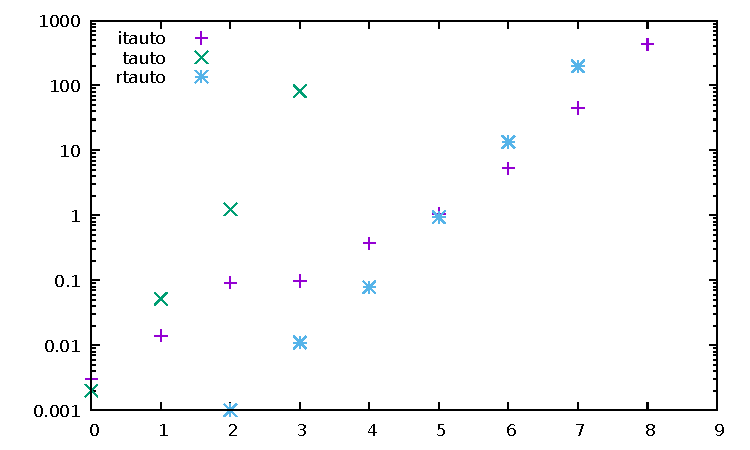
\includegraphics[width=0.45\linewidth]{images/pigeon_tac.pdf}}
  \qquad
  \subfloat[\centering Running time of type-checking.]
  {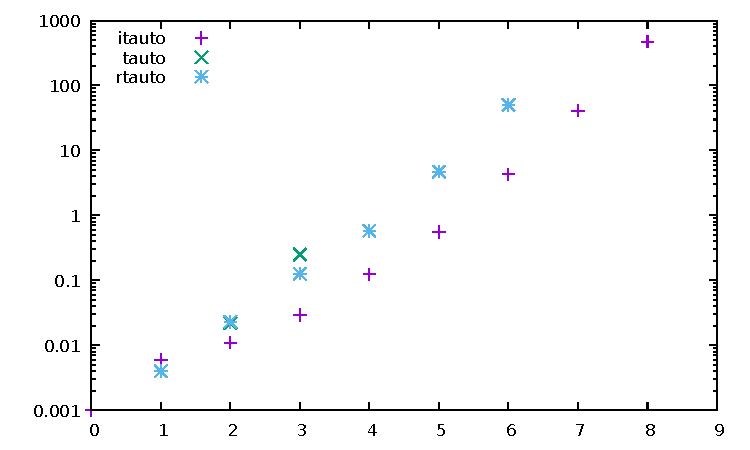
\includegraphics[width=0.45\linewidth]{images/pigeon_qed.pdf}}
  \caption{Pigeon Hole for \icoq{itauto}, \icoq{tauto} and \icoq{rtauto}}
  \label{fig:pigeon}
\end{figure}
For \icoq{itauto}, the time for running the tactic and type-checking
time (\icoq{Qed} time) are similar.  As we perform a pure proof by
reflection, this is not surprising.  Tough \icoq{itauto} scales
slightly better, the running time are similar to \icoq{rtauto} which
only performs proof by reflection to check certificates.
%
\icoq{tauto} is the least scalable and reaches the timeout quickly.
%
\icoq{rtauto} exhausts its memory quota when checking its certificate for 7 pigeons.
\icoq{itauto} reaches the time limit of 1000s for 9 pigeons.

\subsection{On existing developments}

We have benchmarked \icoq{itauto} against the existing Coq tactics
\icoq{tauto} and \icoq{intuition} for the
Bedrock2\footnote{https://github.com/mit-plv/bedrock2} and
CompCert\footnote{\url{https://github.com/AbsInt/CompCert}}
developments.
%
We have replaced calls to \icoq{tauto} and \icoq{intuition tac} for
\icoq{tac} $\in$ \{\icoq{idtac}, \icoq{assumption},
\icoq{discriminate}, \icoq{congruence}, \icoq{lia}, \icoq{auto},
\icoq{eauto} \}.
%
We have ruled out calls to \icoq{intuition} when they generate sub-goals.
%
In  terms of  completeness, \icoq{itauto}  is able  to solve  the vast
majority  of the  goals.  One
representative case of failure is given in Example~\ref{exa:counter}. 
\begin{example} The following goal is solved by \icoq{intuition congruence}.
  \label{exa:counter}
  \begin{minted}{coq}
    Goal true = true <-> (Z -> (False <-> False)).
  \end{minted}
  Yet, \icoq{itauto congruence} fails because \icoq{Z} (\emph{i.e.},
  the type of integers) has type \icoq{Set} and therefore the whole
  expression \icoq{Z -> (False <-> False)} is reified as an opaque
  atomic proposition. Our solution is to call \icoq{itauto}
  recursively \emph{i.e.}, \icoq{itauto (itauto congruence)} so that
  an hypothesis \icoq{x:Z} is explicitly introduced. The same approach
  works in case of goals with inner universal quantifiers.
\end{example}
For a few instances, we also strengthen the leaf tactic \emph{e.g.},
\icoq{idtac} by \icoq{reflexivity}, and, \icoq{discriminate} by
\icoq{congruence}. This is due to the fact that \icoq{intuition}
implicitly calls \icoq{reflexivity} and that theory reasoning
sometimes introduces negations which fool the \icoq{discriminate} tactic.

After modification, Bedrock2 performs 1621 calls to \icoq{itauto}. For
almost 50\% of the goals, the running time differs by less than 1ms and
\icoq{itauto} outperforms the historic tactics for 13\% of the
cases. Overall, \icoq{itauto} is slower and there is an average slowdown of 66\%.
Yet, all the calls are quickly solved; the slower goal solved in 0.4s.

CompCert performs 924 calls to \icoq{itauto}.  For almost 55\% of the
goals, the running time also differs by less than 1ms. \icoq{itauto}
outperforms the  historic tactics for 16\% percent of the
goals. Yet, when \icoq{itauto} is faster it can be by several orders
of magnitudes: the 16\% percent of goals are solved almost 20 times
faster by \icoq{itauto}.
%
For instance, the maximum running time of \icoq{tauto} is 7.26s to be
compared to 0.018s for \icoq{itauto}. Overall, \icoq{itauto} performs
better with a speedup of 2.4 for solving all the goals.

In summary, the results are mixed and it is hard to draw definitive conclusions.
%
It seems that \icoq{itauto} shows a decisive advantage for goals that
are very slow with the existing tactics.
As also shown by the Pigeon Hole experiment, this would indicate a better scalability.
%
It would not be surprising for \icoq{itauto} to be slower on simple goals where
the overhead of setting up the proof by reflection cannot be amortised.
%
Yet, more work is needed to precisely understand the origin of the
slowdown and how the time is spent between the different proof tasks:
SAT solver, theory reasoning and proof by reflection.

\section{Related Work}
\label{sec:related-work}

%%\subsection{Interface with external provers.}
%%An appealing approach to increase the automation of proof-assistants
%%is to delegate proof search to external provers and reconstruct a
%%proof inside the proof-assistant.
%. Yet, their results
%are not trusted by \emph{skeptical} proof
%assistants~\cite{HarrisonT98}. Once the external prover succeeds, its
%output is analysed in order to guide the proof reconstruction running
%inside the proof assistant.

For propositional logic, Weber and Amjad~\cite{WeberA09} for HOL
theorem provers and Armand \emph{et al.}~\cite{ArmandGST10} for Coq
show how to efficiently validate resolution proofs that can be
generated by modern SAT solvers using Conflict Driven Clause Learning
(\emph{e.g.} zChaff~\cite{MoskewiczMZZM01}).
%
Satisfiability Modulo Theory (SMT) solvers (\emph{e.g.},
veriT~\cite{BoutonODF09}, Z3~\cite{MouraB08} ,
CVC4~\cite{DetersR0BT14}) produce proof artefacts. Böhme and
Weber~\cite{BohmeW10} show how to efficiently perform proof
reconstruction for HOL provers. Armand~\emph{et
  al.}~\cite{ArmandFGKTW11} and Besson~\emph{et al.}~\cite{BessonCP11}
extract proof certificates from SMT proofs that are validated in Coq.
%
Sledgehammer~\cite{BlanchetteBP13} interfaces Isabelle/HOL with a
variety of provers; Metis~\cite{Hurd03first-orderproof,PaulsonS07} is
in charge of performing proof reconstruction.
%
We follow a different approach and verify a SAT solver interfaced with
the tactics of Coq. What we loose in efficiency, we gain in flexibility.

Claessen and Ros{\'{e}}n~\cite{ClaessenR15} build a prover for
intuitionistic logic on top of a black-box SAT solver. Their
implementation is more efficient than ours but is not integrated
inside a proof-assistant. 
% 
Lescuyer and
Conchon~\cite{lescuyer08tphol,LescuyerC09} formalise a reflexive SAT
solver for classical logic. Their implementation features a lazy
definitional CNF that is not fully exploited because of the lack of
hash-consing. Compared to ours, their SAT solver performs neither lazy
unit propagation nor backjumping.
%
Blanchette \emph{et al.}~\cite{BlanchetteFLW18} formalise a Conflict
Driven Clause Learning (CDCL) SAT solver and derive a verified
implementation. Using this framework, Fleury, Blanchette and
Lamich~\cite{FleuryBL18} derive an imperative implementation using
watched literals. Our implementation has less sophisticated features
but is integrating as a reflective proof procedure and allows to
perform theory reasoning.

%%These works validate proofs of remarkable size and are almost push
%%button technologies. This has the downside that users has little
%%leverage to guide the proof search. In an interactive setting, domain
%%specific proof tactics are often very effective. This expert knowledge
%%is hard to convey to external provers.
%%%
%%For Coq, there is the additional hassle that automated provers do not
%%with in intuitionistic logic.


\section{Conclusion and Future Work}
\label{sec:conclusion}

We have presented \icoq{itauto} a reflexive tactic for intuitionistic
propositional logic which can be parametrised by user-provided tactics.
%
The SAT solver is optimised to leverage classical reasoning when
possible thus limiting, when possible, costly intuitionistic reasoning.
%
Our SAT solver has several features found in modern SAT solver. Yet,
the implementation could be improved further. A first improvement
would be to generate more sophisticated learnt clauses. This could be
done by attaching to each clause, not only the needed literals, but
also the performed unit propagations. Another improvement would
be to use primitive persistent arrays (available since Coq 8.13)
allowing to implement efficiently more imperative algorithms
\emph{e.g.},  2-watched literals.




\bibliography{biblio}
\end{document}

%%% Local Variables:
%%% mode: latex
%%% TeX-engine: xetex
%%% TeX-master: t 
%%% TeX-command-extra-options: "-shell-escape"
%%% mode: flyspell
%%% ispell-local-dictionary: "british"
%%% End: